\chapter{Produktdaten}

\textbf{/D203/} Für jedes Neuronale Netz werden die folgenden Daten gespeichert: 

\begin{tabular}{cl}
(1) & id \\[0.2cm]
(2) & Name des Neuronalen Netzes\\[0.2cm]
(3) & Beschreibung des Neuronalen Netzes\\[0.2cm]
(4) & Typ Neuronalen Netzwerkes (Prod, Test)\\[0.2cm]
(5) & alle Ids der im Neuronalen Netz enthaltenen Layer.  
\end{tabular}

Für jeden Layer eines Neuronalen Netzes werden die folgenden Daten gespeichert: 

\begin{tabular}{cl}
(1) & id \\[0.2cm]
(2) & Dimension (in x- und y-Richtung) des Layers \\[0.2cm]
(3) & alle Ids der im Layer enthaltenen Knoten.
\end{tabular}

Für jeden Knoten eines Layers werden die folgenden Daten gespeichert: 

\begin{tabular}{cl}
(1) & id \\[0.2cm]
(2) & der Bias \\[0.2cm]
(4) & die Aktivierungsfunktion.
\end{tabular}

Für jedes Kindaxon eines Knotens werden die folgenden Daten gespeichert: 

\begin{tabular}{cl}
(1) & das Gewicht eines Axons \\[0.2cm]
(2) & die Elternknotenid \\[0.2cm]
(3) & die Kindknotenid \\[0.2cm]
\end{tabular}

Zur Persistenz der gesamten oben aufgeführten Daten eines Neuronalen Netzes werden die in Abb. \ref{fig_dbClassdiagram} dargestellten Datenstrukturen verwendet und in einer MongoDB abgelegt. 
\begin{figure}[h]
\begin{center}
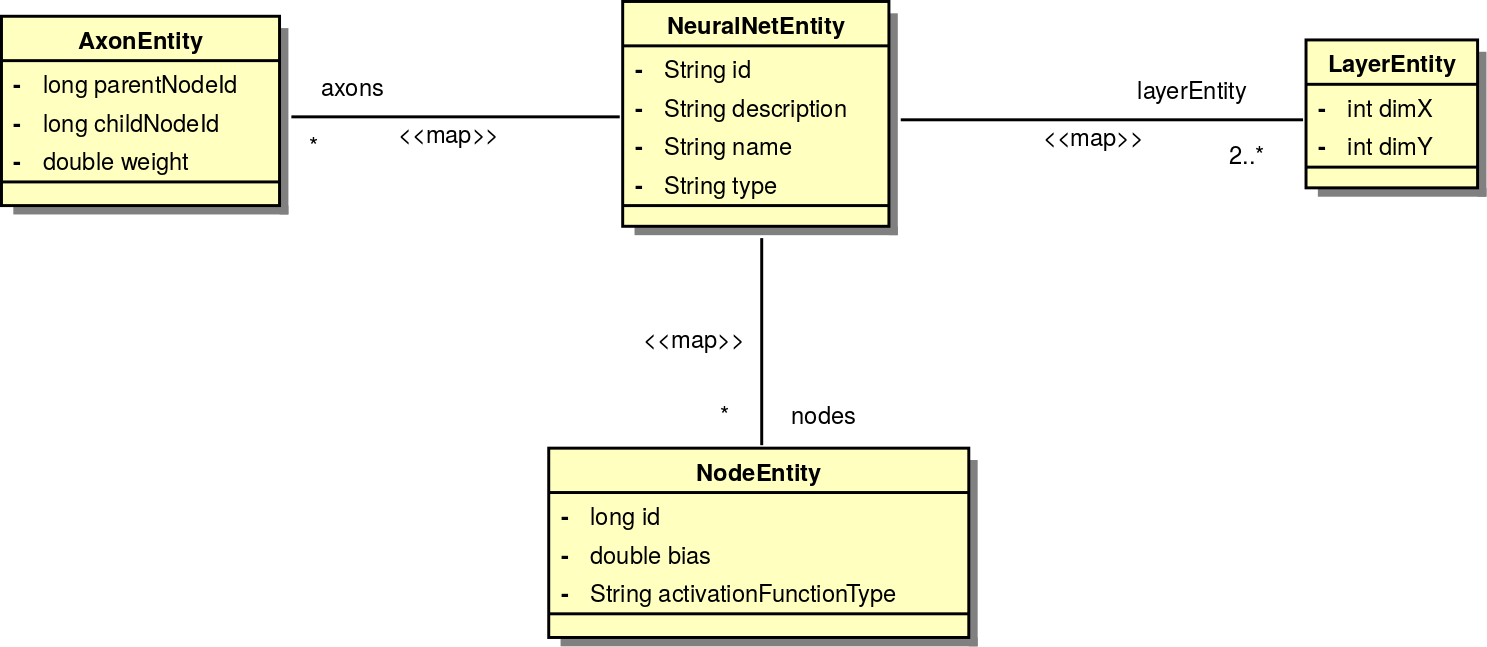
\includegraphics[width=\textwidth]{Abbildungen/UML/jan/datenBankKlassendiagramm.png}
\caption{Klassendiagramm der zur Persistierung eines Neuronalen Netzes benötigten Datenstrukturen.}
\label{fig_dbClassdiagram}
\end{center}
\end{figure}
Es ist zu beachten, dass die Objekt dabei nicht als unabhängige, in Beziehung stehende Entitäten\footnote{Dies entspräche dem Vorgehen für eine Relationale Datenbank. Durch die vielen zirkulären Referenzen ist dieser Zugang nicht geeignet} in der Datenbank sondern als ein einziges Json-Objekt abgelegt werden. 
